\section{Diskussion}
\label{sec:Diskussion}
Die Ergebnisse aus Abschnitt \ref{sec:Auswertung} sowie die Literaturangabe und die Abweichung zu selbigen sind in Tabelle~\ref{tab:ergebnisse} aufgeführt.
\begin{table}[htp]
	\begin{center}
		\begin{tabular}{l
                        S[table-format=4.0(3)]
                        S[table-format=1.6(6)]
                        S[table-format=4.0]
                        S[table-format=1.7]
                        S[table-format=2.1]
                        S[table-format=2.1]}
			\toprule
			& {$T_{\sfrac{1}{2}}[\si{\second}]$}
            & {$\lambda[\si{\per\second}]$}
            & {$T_{\sfrac{1}{2},\text{lit}}[\si{\second}]$}
            & {$\lambda_{\text{lit}} [\si{\per\second}]$}
            & {$\mathup\Delta T_{\sfrac{1}{2}}[\si{\percent}]$}
            & {$\mathup\Delta\lambda [\si{\percent}]$} \\
			\midrule
			$\ce{^{116}In}$  & 2980(90) & 0.000232(7) 	& 3257 	& 0.0002128 &  8.5 	&  9   \\
			$\ce{^{104}Rh}$  &  380(80)  & 0.0018(4) 	& 260  	& 0.002666  &  46.2 & 32.5 \\
			$\ce{^{104i}Rh}$ &   59(6)   & 0.0118(6) 	& 42.3 	& 0.01639   &  39.4 & 28 \\
			\bottomrule
		\end{tabular}
		\caption{Messergebnisse und deren Abweichung von den Literaturwerten.\cite{pse}}
		\label{tab:ergebnisse}
	\end{center}
\end{table}
Die geringen Abweichungen von unter $\SI{10}{\percent}$ der charakteristischen Größen von der Literaturangabe bei der Messung an Indium zeigen, dass das Verfahren zerlässliche Aussage über die Messgrößen trifft.
Die starken Abweichungen der Messgrößen beider Rhodium-Messungen weisen allerdings auf Probleme hin.
Da es sich bei beiden Rhodium-Isotopen im Vergleich zum Indium um schnell zerfallende Präparate handelt, 
liegt möglicherweise ein systematischer Fehler dadurch vor, 
dass das Präparat nicht mit ausreichend geringer Verzögerung aus dem Aktivator in die Messeinrichtung eingeführt wurde.
Bei weiteren Messungen könnte verstärkt auf eine geringe Verzögerung geachtet werden.
Des Weiteren ist von einer nicht beeinflussbaren statistischen Abweichung auszugehen, da der Zerfall von Atomkernen dem Zufall unterliegt.
Für weiterführende Aussagen hierzu muss das Experiment in dieser Variante wiederholt werden, um die geringen Abweichungen bei der Indium-Messung nicht mit systematischen Fehlern erklären, sondern durch Statistik rechtfertigen zu können.

Der Einfluss der Einteilung in zwei Gruppen ist mögliche Fehlerquelle.
In Abbildungen \ref{fig:rhodium1} und \ref{fig:rhodium2} sind das Diagramm \ref{fig:rhodium} aufgetragen, 
bei denen die Grenze der Gruppen nach links und nach rechts verschoben wurde.
Die aus diesen Alternativen bestimmten Werte für sind Tabelle \ref{tab:alternative} zu entnehmen.
Es lässt sich keine Einteilung finden, bei denen die Messwerte insgesamt verbessert werden.
\begin{table}[htp]
	\begin{center}
		\begin{tabular}{c
						l
                        S[table-format=4.0(3)]
                        S[table-format=1.6(6)]
                        S[table-format=4.0]
                        S[table-format=1.7]
                        S[table-format=2.1]
                        S[table-format=2.1]}
			\toprule
			{Plot}
			&
			& {$T_{\sfrac{1}{2}}[\si{\second}]$}
            & {$\lambda[\si{\per\second}]$}
            & {$T_{\sfrac{1}{2},\text{lit}}[\si{\second}]$}
            & {$\lambda_{\text{lit}} [\si{\per\second}]$}
            & {$\mathup\Delta T_{\sfrac{1}{2}}[\si{\percent}]$}
            & {$\mathup\Delta\lambda [\si{\percent}]$} \\
			\midrule
			1&$\ce{^{104}Rh}$  &  270(30)  & 0.0026(3) 	& 260  	& 0.002666  &  3.8 & 2.5 \\
			&$\ce{^{104i}Rh}$ &   84(6)   & 0.0083(6) 	& 42.3 	& 0.01639   &  98.6 & 49.4 \\
			2&$\ce{^{104}Rh}$  &  500(200)  & 0.0013(5) & 260  	& 0.002666  &  92.3 & 51.2 \\
			&$\ce{^{104i}Rh}$ &   85(6)   & 0.0082(6) 	& 42.3 	& 0.01639   &  101 & 50 \\

			\bottomrule
		\end{tabular}
		\caption{Messergebnisse und deren Abweichung von den Literaturwerten.\cite{pse}}
		\label{tab:alternative}
	\end{center}
\end{table}

\begin{figure}[p]
    \centering
    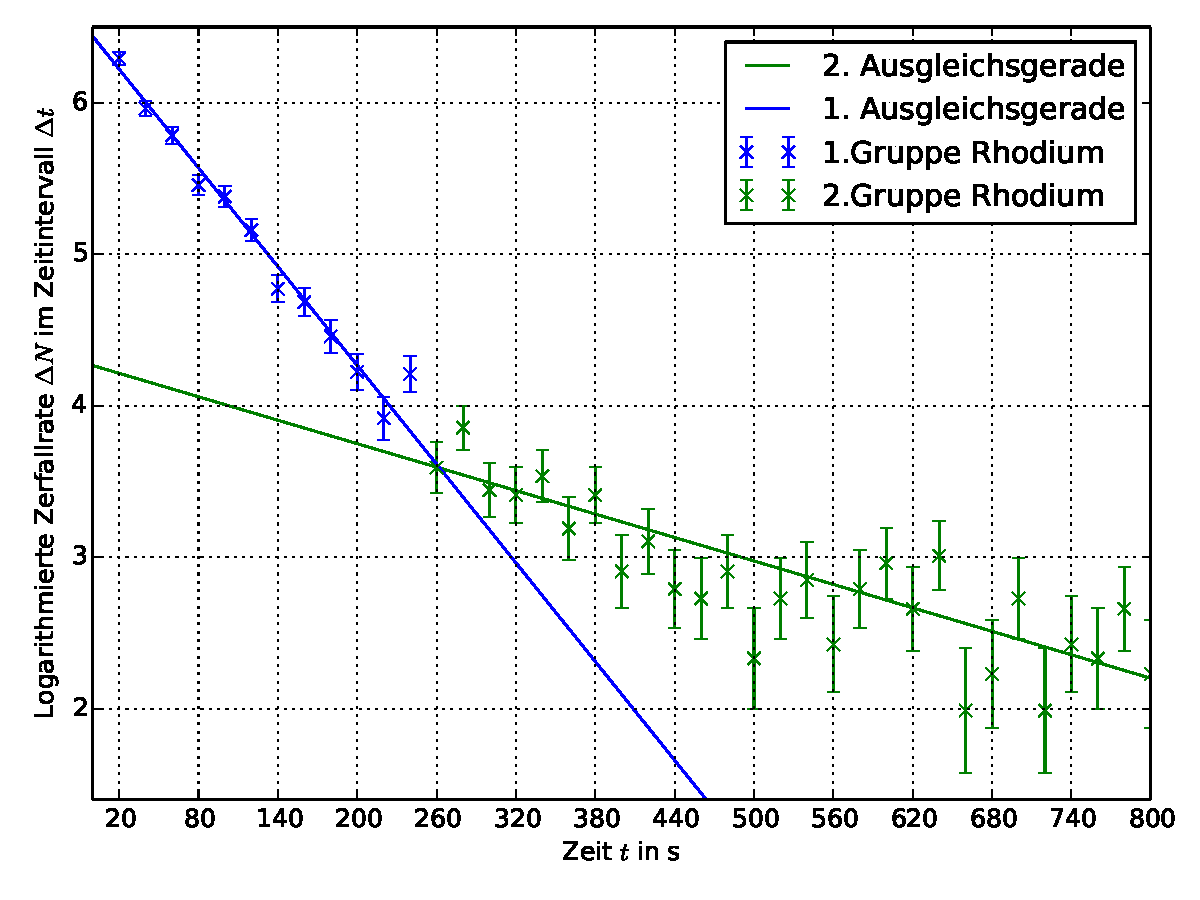
\includegraphics[width=0.8\textwidth]{Bilder/rhodium_1.pdf}
    \caption{Korrigierte und logarithmierte Anzahl der Zerfälle für Indium aufgetragen gegen die Zeit, alternative Einteilung.}
    \label{fig:rhodium1}
\end{figure}
\begin{figure}[p]
    \centering
    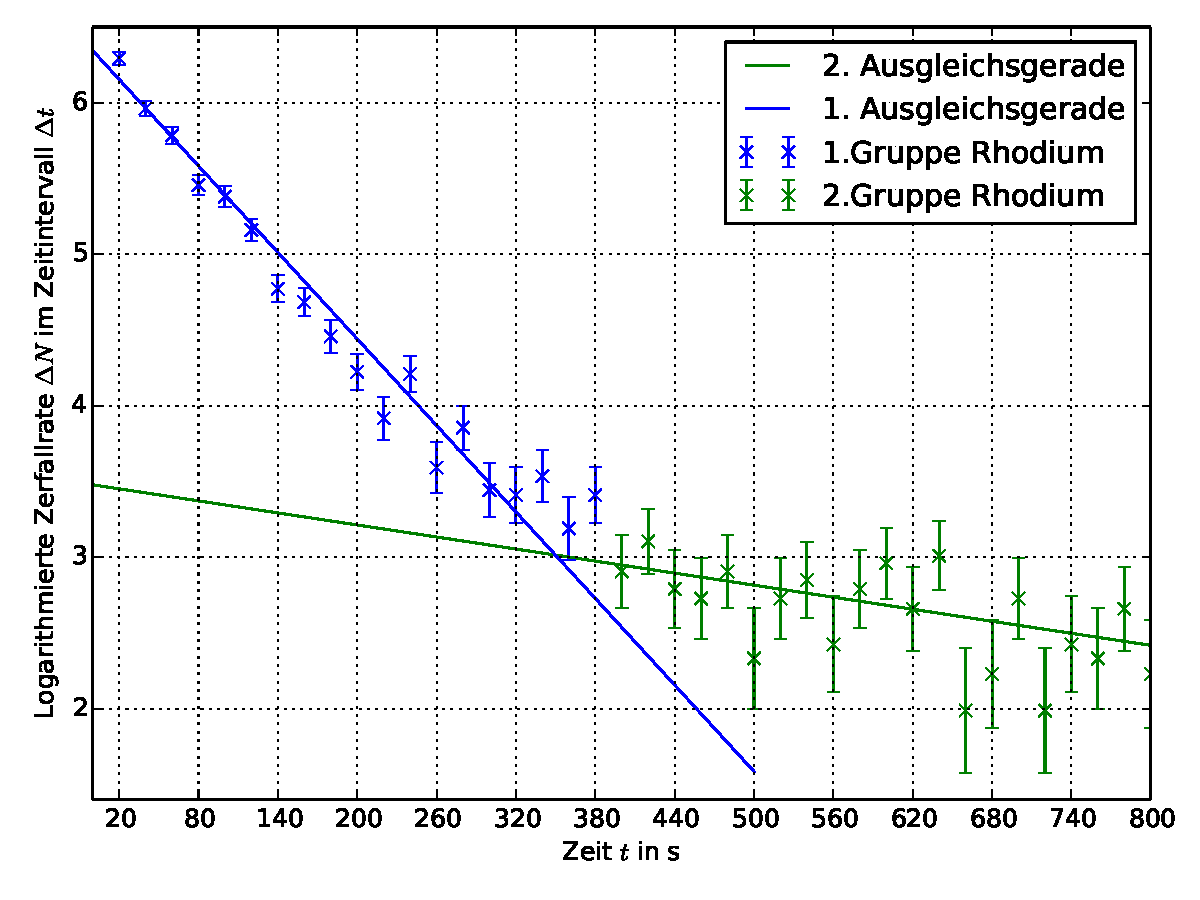
\includegraphics[width=0.8\textwidth]{Bilder/rhodium_2.pdf}
    \caption{Korrigierte und logarithmierte Anzahl der Zerfälle für Rhodium aufgetragen gegen die Zeit, alternative Einteilung.}
    \label{fig:rhodium2}
\end{figure} 